\chapter{Einleitung}

Im folgenden Kapitel werden die Systemkomponenten und deren Zusammenspiel erläutert. Für das Verständnis wird das Aufgabenumfeld in einem abstrakten Kontext dargestellt. Die konkrete Implementierung und detaillierte Analyse werden in den folgenden Kapitel behandelt.

\section{Big Picture}
Zur Übersicht werden die verschiedenen Komponenten des Projektes in einem Big Picture zusammengefasst. Die untenstehende Grafik \ref{fig:bigpicture} ist in drei Abschnitte unterteilt. Im obersten Abschnitt befinden sich alle Geräte, welche Daten erfassen. Diese Aufnahmesysteme bestehen aus der Android TourLiveApp, als Teil dieser Arbeit, sowie dem Android RadioTourSpeaker,  welcher im Rahmen einer Semesterarbeit \cite{radiotourspeaker2012} entwickelt wurde.\\

Im mittleren Teil befinden sich die Serversysteme. Diese bestehen aus dem TourLive Server, welcher die Renndaten empfängt und verarbeitet, sowie dem Device Management Server. Der Device Management Server bietet eine Übersicht über die registrierten Aufnahmesysteme und ermöglicht es, deren Einstellungen zu Verwalten sowie allfällige Fehlerquellen frühzeitig zu erkennen.\\

Der dritte Abschnitt zeigt die Anwendergruppen, die mit den Daten beliefert werden. Dies sind zum einen die Besucher der Webseite des TourLive Servers und zum anderen Drittentwickler, welche auf die öffentliche Schnittstelle zugreifen.\\

Teil dieser Arbeit sind die farblich hervorgehobenen Komponenten: Die Aufnahmesysteme TourLiveApp in Form einer Android App [blau], das Serversystem TourLive Server in Form einer Spring Webapplikation [rot] sowie das Serversystem Device Management Server ebenfalls in Form einer Spring Webapplikation [grün].

\begin{figure}[H]
	\centering
	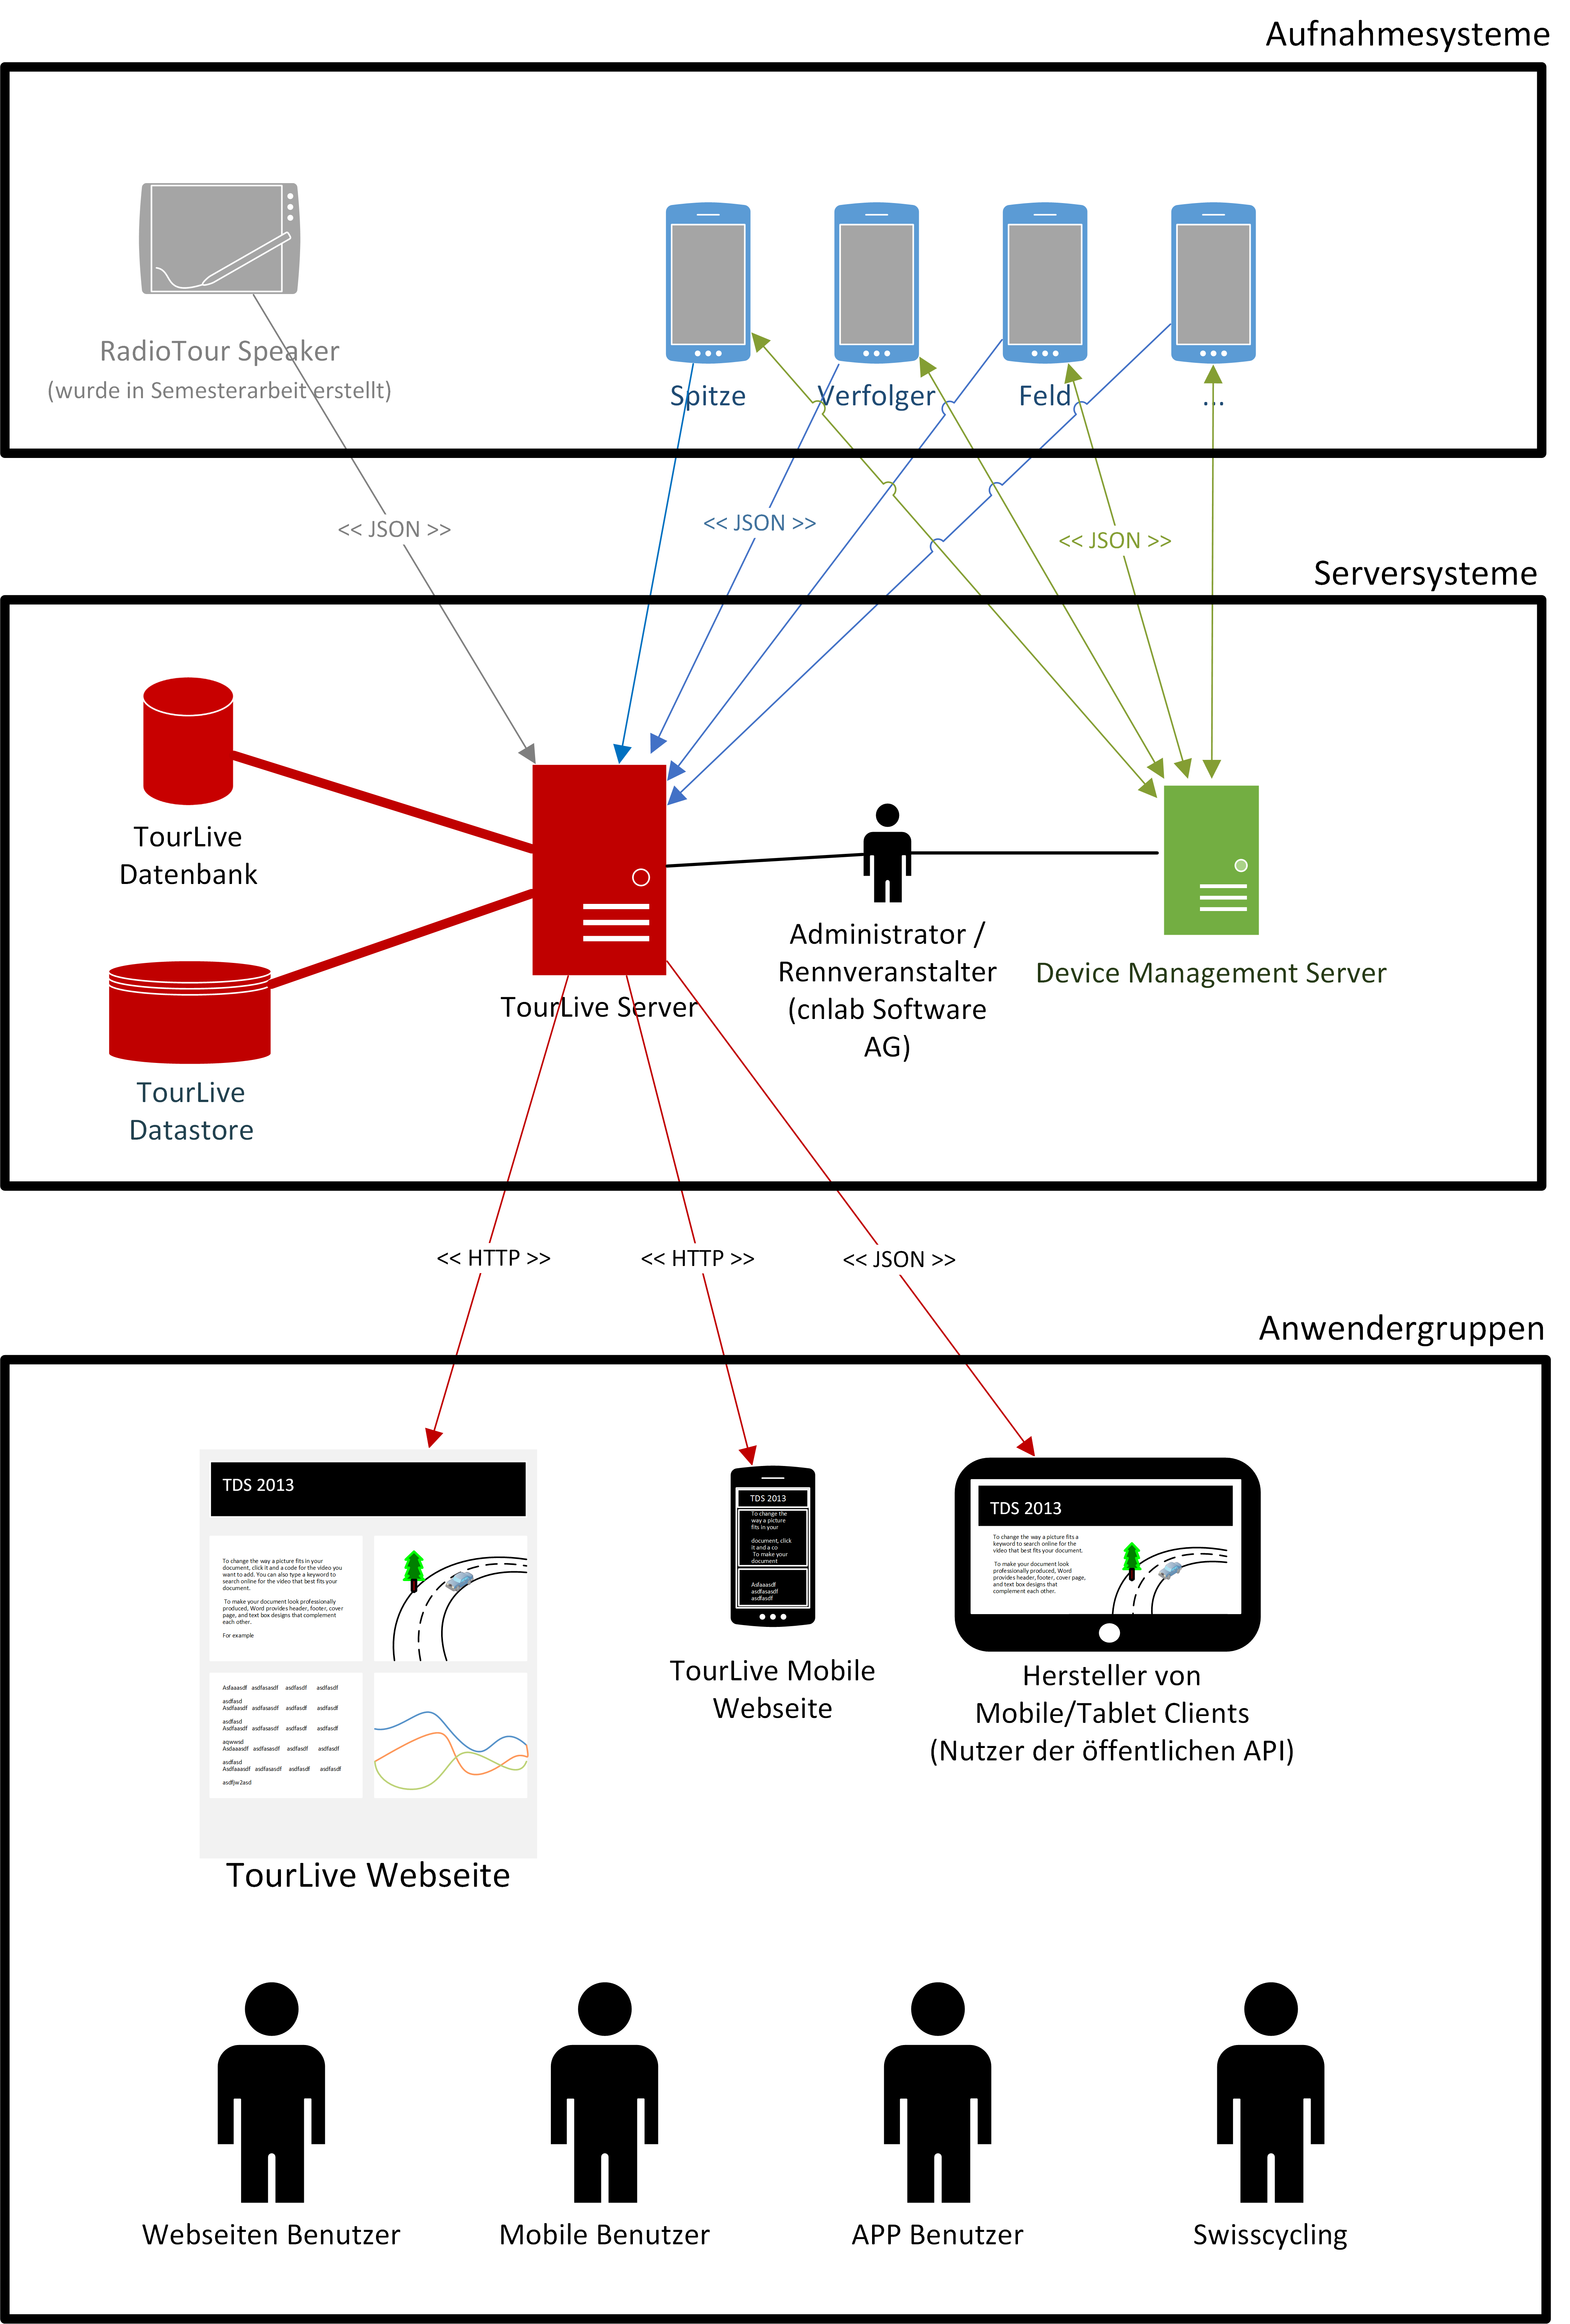
\includegraphics[height=200mm]{images/BigPicture.png}
	\caption{Big Picture}
	\label{fig:bigpicture}
\end{figure}

\pagebreak

\section{Kernelemente}
\subsection{TourLive Server}
Auf der zentralen Webapplikation TourLive Server werden die von den Aufnahmesystemen eingehenden Daten gespeichert, verarbeitet, aufbereitet und weitergegeben. Bild- und Positionsdaten werden in Form einer Webseite für Radsportbegeisterte aufbereitet und in einer öffentlichen Schnittstelle für mögliche Drittentwickler zur Verfügung gestellt. Die Architektur wurde dabei so gewählt, dass das System bei hoher Last gut skaliert. Diese Komponente wird in Kapitel \ref{sec:tourliveserver} genauer behandelt.

\subsection{Device Management Server}
Der Device Management Server hilft dabei, die aktiven Aufnahmegeräte zu verwalten. Es ersetzt das existierende Portal, welches nur wenig Funktionalität besitzt. Sollte der Device Management Server nicht verfügbar sein, sind die Aufnahmegeräte trotzdem einsatzfähig, da die Einstellungen auch lokal am Smartphone vorgenommen werden können. Auf den Device Management Server wird im Kapitel \ref{sec:devmgmtsrv} eingegangen.

\subsection{Aufnahmesystem}
Ein weiterer Bestandteil des Endsystems ist das Aufnahmesystem. Es ersetzt die Symbian App auf den Nokia Handys. Periodisch werden alle gesammelten Daten vom Aufnahmesystem an den TourLive Server übermittelt. Ebenfalls periodisch werden die Einstellungen vom Device Management Server abgeholt und der Gerätestatus mitgeteilt. Werden die Einstellungen lokal verändert, so werden die veränderten Einstellungen an den Device Management Server übertragen. Im Kapitel \ref{sec:androidaufnahmesystem} wird diese Komponente detailliert beschrieben.